\begin{figure}[htbp]
\centering
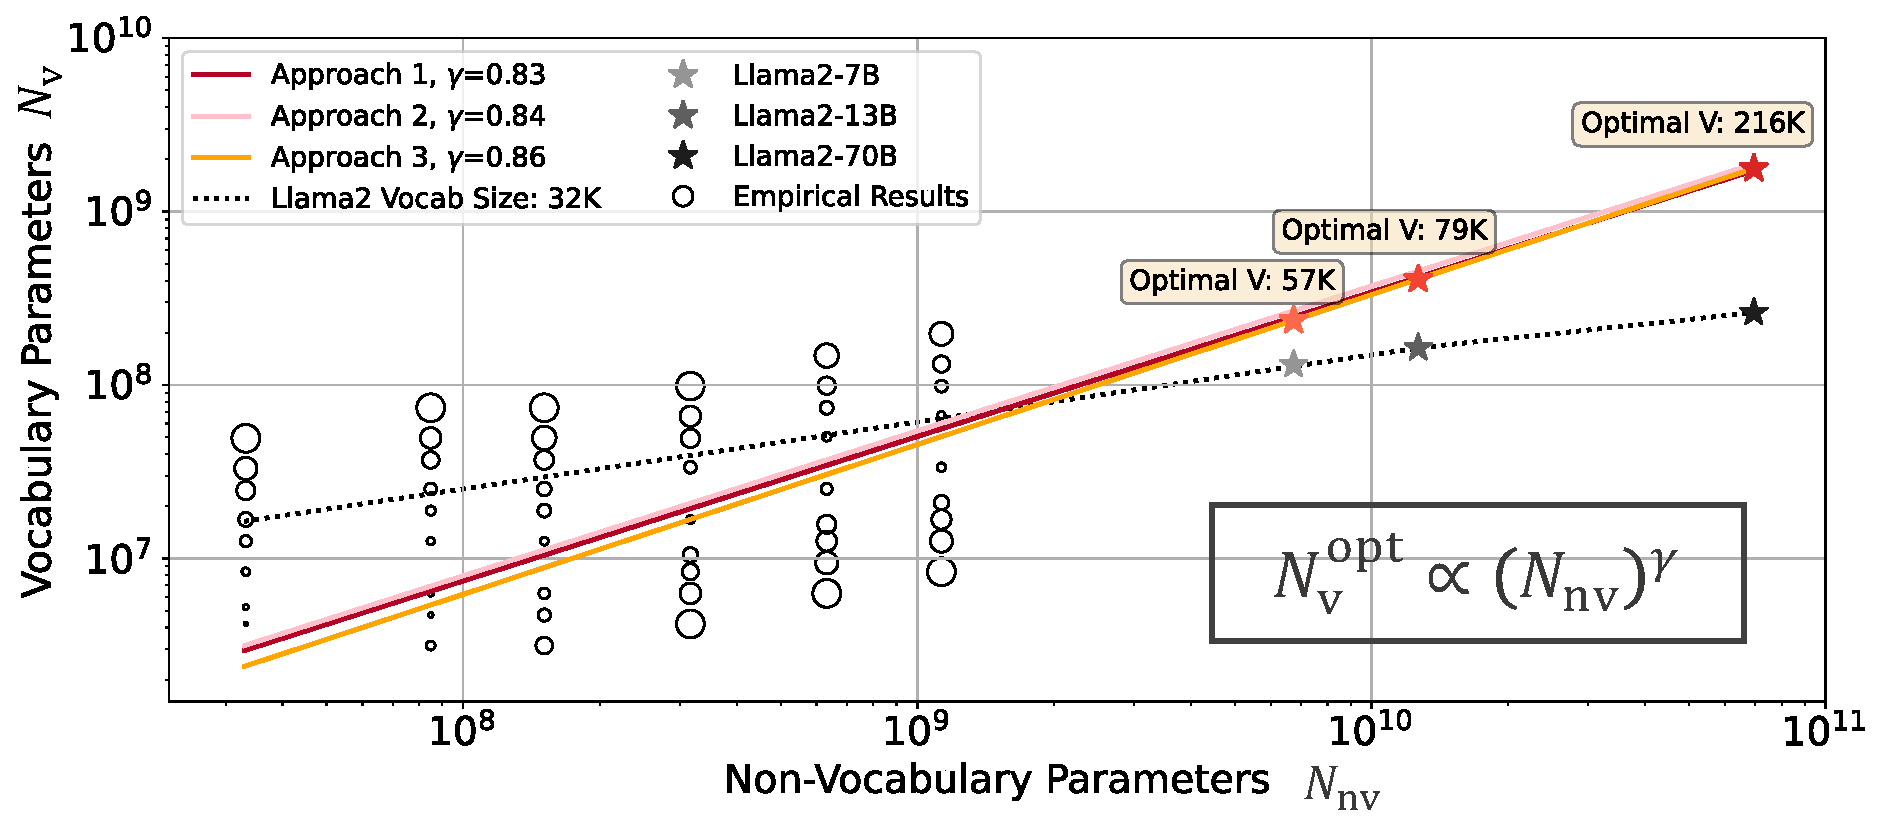
\includegraphics[width=.95\textwidth]{figures/figure_1_left_scaling_v9.pdf}
\caption{The relationship between non-vocabulary parameters $N_{\rm nv}$ and the corresponding optimal vocabulary parameters $N_{\rm v}^{\rm opt}$ follows a power law, where $N_{\rm v}^{\rm opt}$ should be scaled slower than $N_{\rm nv}$ as $\gamma < 1$. Empirical results align with predictions of our proposed approaches, with larger circles indicating higher loss values. Here $V$ refers to the vocabulary size i.e. the number of distinct tokens.}
\label{fig:intro}
\end{figure}

\section{Introduction}
\label{sec:intro}

Large language models (LLMs) achieve remarkable performance by pre-training on vast text corpora using massive computational resources~\citep{achiam2023gpt}. Extensive prior work on LLMs has focused on deriving so-called scaling laws: a set of empirical formulas to predict how model performance scales, mainly as computing floating-point operations (FLOPs), model parameters, and quantity of training data change~\citep{kaplan2020scaling,hoffmann2022training,tay-etal-2023-scaling,aghajanyan2023scaling,muennighoff2024scaling,scao2022language}. These works show that power-law fits can effectively predict language modeling loss and by extension downstream performance~\citep{gadre2024language,ruan2024observational}. However, these scaling laws usually disregard the impact of the vocabulary size. For example, in~\citet{kaplan2020scaling} only non-vocabulary parameters are considered in their predictive formula.
This negligence has resulted in substantial variability in the vocabulary size of current LLMs.
For instance, Llama2-7B employs a vocabulary size of 32K~\citep{touvron2023llama}, while Gemma-7B~\citep{team2024gemma} adopts a much larger vocabulary size of 256K despite both having a similar number of total parameters. This variability in vocabulary sizes across LLMs raises the research question: \textit{What is the compute-optimal vocabulary size for a LLM?}  \looseness=-1
  
The vocabulary size affects performance non-trivially. Intuitively, the optimal vocabulary size should neither be too large nor small. A larger vocabulary size improves tokenization fertility, i.e., splitting sentences into fewer tokens, thereby improving the tokenization efficiency.
Additionally, a larger vocabulary enables the model to capture a wider range of concept. However, the risk of under-fitting for rare tokens increases with larger vocabulary sizes, especially in the data-constrained regime~\citep{muennighoff2024scaling,villalobos2022will}. Thus, the optimal vocabulary size needs to be determined by taking the training data and the non-vocabulary parameters into account. \looseness=-1


In this paper, we show that the effect of vocabulary on scaling laws has been underestimated, and we quantify the effect to derive a prediction for {the optimal vocabulary size}. We first introduce a normalized loss formulation to ensure a fair comparison across models with varying vocabulary sizes. Utilizing the normalized loss function, we analyze and discuss the underlying rationale behind the existence of an optimal vocabulary size, which depends on the available computational budget. 


To predict the optimal vocabulary size given a compute budget, we propose three approaches. {\textbf{Approach 1 (Estimating power laws via IsoFLOPs)}:} We pre-train models with non-vocabulary parameters ranging from 33M to 1.13B, with groups of models that share the same FLOPs (``IsoFLOPs'') but varying vocabulary configurations. Then, we fit power laws relating FLOPs to non-vocabulary parameters, vocabulary parameters, and training data, respectively. Our analysis reveals that the optimal vocabulary parameters exhibit a power-law growth with respect to the computational budget, however, at a slower rate than non-vocabulary parameters, as shown in~\autoref{fig:intro}. {\textbf{Approach 2 (Derivative-based Estimation)}:} We introduce a derivative-based method that estimates the optimal vocabulary size by using the derivative of FLOPs w.r.t. the vocabulary size and finding the corresponding zero solution. {\textbf{Approach 3 (Parametric Fit of Loss Formula)}:} We modify Chinchilla scaling laws~\citep{hoffmann2022training} to incorporate vocabulary and fit the resulting formula on our models to predict the normalized loss function based on non-vocabulary parameters, vocabulary parameters, and the amount of training characters jointly. While the prior two approaches are limited to compute-optimal settings, this approach also allows us to determine the optimal vocabulary when the allocation is suboptimal i.e. the model parameters are either trained for too many tokens (``overtrained'') or for too few tokens (``undertrained''). Overtraining is very common~\citep{gadre2024language}, such as Llama 2 7B~\citep{touvron2023llama} which was trained for 2 trillion tokens, significantly more than the compute-optimal allocation of a 7 billion parameter model of around 150B tokens.

\begin{figure}[t]
\centering
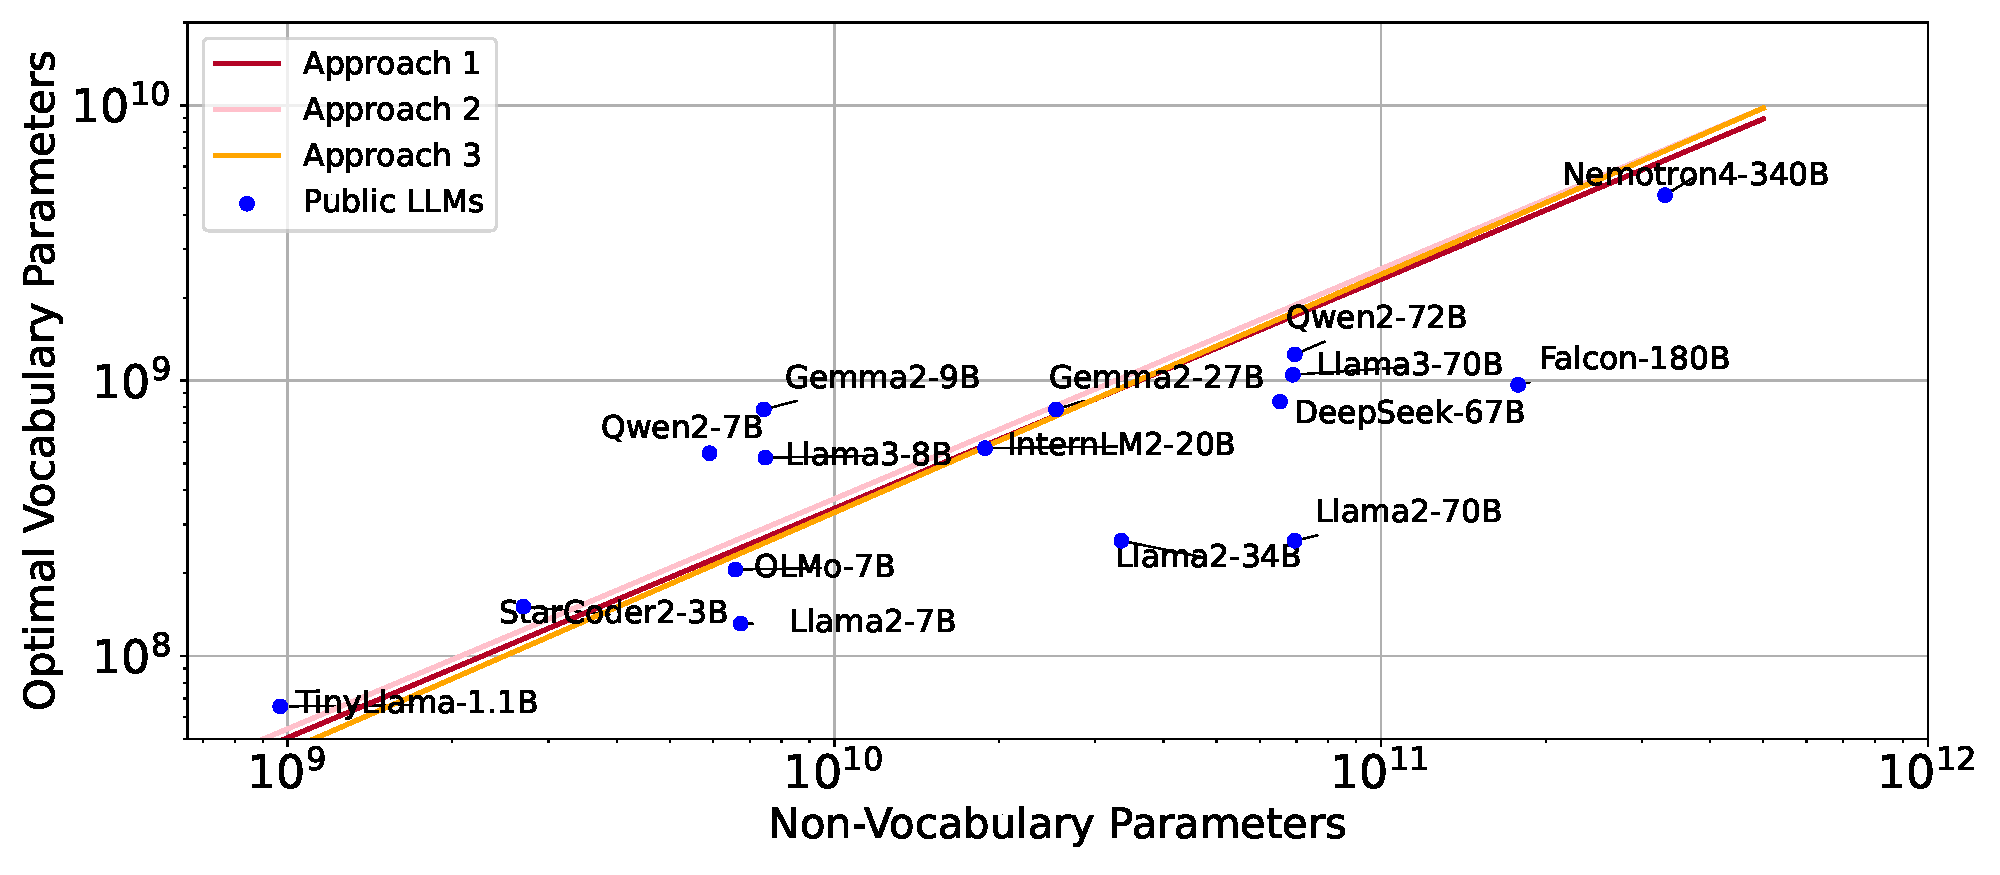
\includegraphics[width=0.95\textwidth]{figures/figure_1_right_v6.pdf}
\caption{Vocabulary parameters of popular LLMs and predicted optimal vocabulary parameters at a \textbf{compute-optimal number of training tokens}. Most current LLMs have suboptimal vocabulary parameters due to vocabulary sizes, which are smaller than the predicted optimal values. Among the current models, {StarCoder2-3B}, {OLMo-7B}, {InternLM2-20B}, and {Gemma2-27B} have vocabulary sizes that come closest to the optimal allocation for their respective model sizes.}
\label{fig:motivation2-scaling-Nnv}
\end{figure}

As shown in \autoref{fig:intro}, we observe that the relationship between non-vocabulary parameters $N_{\rm nv}$ and their correspondng optimal vocabulary parameters $N_{\rm v}^{\rm opt}$ follows a power law, according to all of our approaches. 
Our prediction also suggests that vocabulary parameters should be scaled slower than non-vocabulary parameters, i.e., $N_{\rm v}^{\rm opt} \propto N_{nv}^{\gamma}$ where $\gamma \approx 0.83 < 1$. 
Nevertheless, most of existing LLMs~\citep{li2023starcoder,yang2024qwen2technicalreport,team2024gemma,metallama3blog,almazrouei2023falcon,groeneveld2024olmo,cai2024internlm2technicalreport,deepseekllm2024,nvidia2024nemotron4,zhang2024tinyllama} neglect the importance of vocabulary and allocate less vocabulary parameters than the suggestions, shown in \autoref{fig:motivation2-scaling-Nnv}. 
Note that we assume that the amount of training data for these models is optimally distributed according to \citet{hoffmann2022training}.
Considering that several LLMs are trained on substantially more data than optimal ones (e.g., Llama2), the optimal vocabulary sizes would likely be larger than currently estimated.

Finally, we empirically verify our predictions on models with 3B parameter models. By using our approach to predict the expected vocabulary size in various practical cases when (1) the training data is insufficient (``undertraining''); (2) the training data is equally scaled with the model parameters, following the Chinchilla laws (``compute-optimal training'')~\citep{hoffmann2022training}; (3) the training data is overly sufficient like in Llama~\citep{touvron2023llama} (``overtraining''). The results show that models with our suggested vocabulary sizes steadily outperform baselines adopting commonly used vocabulary configurations under the same FLOPs budget.
Our research underscores the overlooked importance of vocabulary and the need to jointly consider the vocabulary size, model parameters, and training data for effective scaling.
\looseness=-1
